\documentclass[12pt, spanish]{article}
\usepackage[spanish]{babel}
\selectlanguage{spanish}

% estilo personalizado
\usepackage{src/estilo}


\begin{document}

% Página de titulo

%%%%%%%%%%%%%%%%%%%%%%%%%%%%%%%%%%%%%%%%%%%%%%%%%%%%%%%%%%%%%%%%%%%%%%%%%%%%%%%%%%%%%%%%%

\begin{titlepage}
    \centering
    \vspace*{-2cm}
    
\includegraphics[scale = 0.50]{ugr.png}\\[0.3 cm]
    %\textsc{\LARGE Universidad de Granada}\\[2.0 cm]
    \textsc{\large Trabajo Fin Grado}\\[0.5 cm]
    \textsc{\large Grado en Ingeniería Informática}\\[0 cm]
    \rule{\linewidth}{0.2 mm} \\
    { \Large \bfseries \thetitle}\\
    \rule{\linewidth}{0.2 mm} \\[1 cm]

    \begin{minipage}{\textwidth}
		\begin{center}
			\large
			\emph{Autor:} \theauthor \hspace{0.5 cm}
			\emph{DNI:} 77021623-M \vspace{0.2cm} \\
			\emph{Director:} Óscar Cordón García \\
			\emph{Director:} Sergio Damas Arroyo \\
		\end{center}
    \end{minipage}\\[0.5cm]
	 
\includegraphics[scale = 0.20]{logo_etsiit.png}\\[0.3 cm]
    {\large \thedate}\\[0.5cm]
	 \url{https://github.com/advy99/TFG/}
    \doclicenseThis
\end{titlepage}


% resumen antes del indice

\clearpage
\begin{center}
	{\large\textbf{\thetitle}}


	\theauthor
\end{center}

\textbf{Palabras clave:} Antropología Forense, Estimación de la Edad a partir de Restos Óseos, Inteligencia Artificial Explicable,
Aprendizaje Automático, Programación Genética, Metaheurísticas.

\textbf{Resumen:}

La estimación de la edad, tanto de personas fallecidas como vivas, es una de las tareas más importantes en la antropología forense. Actualmente este proceso de estimación de la edad se basa en analizar ciertas características como la apariencia, morfología o patrones de osificación en los restos óseos de los individuos. Entre los distintos métodos utilizados destaca la sínfisis púbica debido a su alta fiabilidad. Este proceso se realiza de forma manual, aunque en los últimos años han aparecido diversos trabajos que intentan automatizar la estimación de la edad a partir de restos óseos. Los resultados de estos métodos son demasiado complejos para servir de apoyo a los forenses de cara a mejorar y perfeccionar la técnica, a pesar de conseguir unas estimaciones aceptables.

Por este motivo, uno de los últimos enfoques aplicados sugiere buscar métodos de inteligencia artificial explicable, permitiendo obtener modelos sencillos y facilmente entendibles. Esto puede conllevar una peor estimación por parte del modelo, pero el objetivo final no es automatizar por completo la tarea, si no servir de apoyo al forense y de esta forma facilitar su trabajo a la vez que se puede llegar a encontrar detalles que antes no se han tenido en cuenta en el proceso de estimación de la edad.

En este trabajo se partirá de la propuesta de Thomas Wingate Todd en el año 1920, en el que proponía una forma de automatizar la clasificación de restos en diez fases de edad, de cara a trabajar con el conjunto de datos de características de sínfisis púbica del laboratorio de Antropología Física de la Universidad de Granada.

Este problema se trata de un problema complejo de aprendizaje automático debido a que el tamaño del conjunto de datos es muy pequeño, tiene una gran cantidad de características y está altamente desbalanceado. Sumado a esto, tenemos como objetivo que el modelo final sea simple de cara a dar con un buen resultado que los forenses sean capaces de aplicar.

Para cumplir estos objetivos, en este trabajo se tratarán diversas técnicas para balancear los datos, reducir su dimensionalidad y se tratarán diversos enfoques de algoritmos genéticos de cara a obtener un modelo simple.

Para comenzar se utilizarán algoritmos basados expresiones matemáticas de cara a, con una sola fórmula, estimar la edad de cada individuo, primero explorando y entrenando el enfoque clasico de Programación Genética, mejorarlo añadiendo un algoritmo genético a la Programación Genética (GA-P) con el objetivo de suplir algunos de sus problemas, y finalmente utilizando sistemas basados en gramáticas para obtener reglas facilmente interpretables.

\newpage


\begin{center}
	{\large\textbf{\thetitleEN}}


	\theauthor
\end{center}

\textbf{Keywords:} Forensic anthropology, Age estimation from bone remains, Explainable Artificial Intelligence,
Machine Learning, Genetic Programming, Metaheuristics.

\textbf{Abstract:}

Age estimation, both for deceased and living people, is one of the most important tasks for forensic anthropology. Currently this process of age estimation is based on analyzing certain characteristics such as appearence, morphology or ossification patterns in the skeletal remains of individuals. Among the different methods used, the pubic symphysis stands out due to its high reliability. This process is performed manually, although in recent years there have been several studies that attempt to automate age estimation from bone remains. The results of these methods are too complex to support forensic scientists at improving and refining the technique, despite achieving acceptable estimates.

For this reason, one of the latest applied approaches suggests searching for explainable artificial intelligence methods, allowing to obtain simple and easily understandable models. This may lead to a worse estimation by the model, but the ultimate goal is not to fully automate the task, but to support the forensic scientists and thus facilitate his work while finding details that have not been previously taken into account in the age estimation process.

In this work we will start from Thomas Wingate Todd's proposal in 1920, in which he proposed a way to automate the classification of remains in ten age stages, in order to work with the dataset of pubic symphysis characteristics of the Physical Anthropology Laboratory of the University of Granada.

This problem is a complex machine learning problem beacuse the dataset size is very small, has a large amount of features and is highly unbalanced. In addition to this, we aim to keep the final model simple in order to give a good result that forensic scientists will be able to apply.


To meet these objectives, this work will discuss different techniques to balance the data, reduce its dimensionality and discuss various genetic algorithm approaches in order to obtain a simple model.


To begin with, we will use mathematical expresssion-based algorithms to estimate the age of each individual with a single formula, first exploring and training the classical Genetic Programming approach, improving it by adding a genetic algorithm to Genetic Programming (GA-P) in order to overcome some of its problems, and finally using grammar-based systems to obtain easily interpretable rules.



\newpage

\vspace*{2cm}

\rule{\linewidth}{1 mm} \\[1 cm]

{\large Yo, \textbf{\theauthor}, estudiante del Grado en Ingeniería Informática de la \textbf{Escuela Técnica Superior de Ingenierías Informática y de Telecomunicación de la Universidad de Granada}, con DNI 77021623-M, autorizo la ubicación de la siguiente copia de mi Trabajo de Fin de Grado en la biblioteca del centro para que pueda ser consultada por las personas que lo deseen.}

\vspace{7cm}

Firmado: Antonio David Villegas Yeguas

\vspace{2cm}

Granada, \thedate



\newpage

\vspace*{2cm}

\rule{\linewidth}{1 mm} \\[1 cm]

D. Óscar Cordón García, profesor del Departamento de Ciencias de la Computación e Inteligencia Artificial de la Universidad de Granada.

\vspace{1cm}

D. Sergio Damas Arroyo, profesor del Departamento de Lenguajes y Sistemas Informáticos de la Universidad de Granada.

\vspace{1cm}

\textbf{Informan:}

\vspace{1cm}

Que el presente trabajo, titulado \textbf{Aprendizaje automático de un sistema interpretable de ayuda a la decisión para la estimación de la edad a partir de los huesos del pubis}, ha sido realizado bajo su supervisión por Antonio David Villegas Yeguas, y autorizamos la defensa de dicho trabajo ante el tribunal que corresponda.

\vspace{1cm}

Y para que conste, expiden y firman el presente informe en Granada a \thedate.

\vspace{5cm}

\textbf{Óscar Cordón García.}

\textbf{Sergio Damas Arroyo.}

\newpage

{\Large \textbf{Agradecimientos}}


\pagebreak

% ponemos el estilo de página despues del resumen, firma y agradecimientos

\pagestyle{fancy}


%%%%%%%%%%%%%%%%%%%%%%%%%%%%%%%%%%%%%%%%%%%%%%%%%%%%%%%%%%%%%%%%%%%%%%%%%%%%%%%%%%%%%%%%%

% indice

\tableofcontents
\pagebreak

%%%%%%%%%%%%%%%%%%%%%%%%%%%%%%%%%%%%%%%%%%%%%%%%%%%%%%%%%%%%%%%%%%%%%%%%%%%%%%%%%%%%%%%%%

% secciones

\section{Introducción}

Para este trabajo nos centraremos en resolver un problema real de aprendizaje automático utilizando el conocimiento obtenido a lo largo de las asignaturas de todo el Grado, con especial mención a los conocimientos adquiridos en las asignaturas \textit{Metaheurísticas} y \textit{Aprendizaje Automático}, y explorando nuevas técnicas de inteligencia artificial de cara a complementar dichos conocimientos de forma que se desarrolle un conocimiento en la exploración, formas de trabajo e investigación de nuevas técnicas.

\subsection{Problema a resolver}

De cara a la identificación de cadaveres, una de las tareas clave es la estimación de la edad. Aunque los forenses tenian formas de estimar a que edad murio una persona a partir de sus restos óseos, no existía un método concreto y universal de forma que el forense solo tuviera que seguir ciertas pautas y observar ciertas características de cara a la estimación de la edad.

Por este motivo, en el año 1920, Thomas Wingate Todd publicó un artículo científico \cite{todd} en el que proponía una forma de clasificar en diez rangos de edad los restos óseos de una persona fallecida a partir de ciertas características de la sínfisis púbica, de forma que el proceso de identificación de cadáveres fuera más sencillo para los forenses.

A pesar de ser una publicación de hace más de cien años, este método sigue siendo la base para la estimación de la edad a partir de los restos óseos. La mayoría de técnicas actuales se basan en esta propuesta y se siguen aplicando de forma manual.

El sistema propuesto por Todd se centraba en nueve características, asignándole distintos valores categóricos, de la sínfisis púbica para realizar su clasificación:

\begin{enumerate}
	\item Crestas y surcos: Porosidad regular, muy definidas, poco profundas, restos de surcos o no hay surcos.
	\item Superficie porosa irregular: No, medianamente o sí.
	\item Borde superior: Definido o no definido.
	\item Nódulo óseo: Ausente o presente.
	\item Borde inferior: Definido o no definido.
	\item Borde dorsal: Definido o no definido.
	\item Plataforma dorsal: Ausente o presente.
	\item Bisel ventral: Ausente, en proceso de formación o formado.
	\item Borde ventral: Ausente, parcialmente formado, formado sin excrecencias, formado con pocas excrecencias o formado con muchas excrecencias.
\end{enumerate}

\begin{table}[H]
\resizebox{\textwidth}{!}{%
	\begin{tabular}{|c|c|c|}
	\hline
	Crestas y surcos: Muy definidos & Superficie porosa irregular: Sí & Borde superior: Definido  \\ \hline
	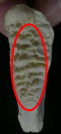
\includegraphics[scale = 0.75]{crestas_surcos_muy_definidos.png}  &   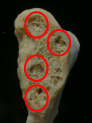
\includegraphics[scale = 0.75]{superficie_porosa_si.png} &  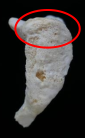
\includegraphics[scale = 0.75]{borde_superior_definido.png}  \\ \hline
	Nódulo óseo: Presente & Borde inferior: No definido & Borde dorsal: Definido \\ \hline
	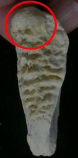
\includegraphics[scale = 0.75]{nodulo_oseo_presente.png} & 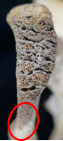
\includegraphics[scale = 0.75]{borde_inferior_no_definido.png} &  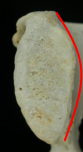
\includegraphics[scale = 0.75]{borde_dorsal_definido.png} \\ \hline
	Plataforma dorsal: Presente & Bisel ventral: En proceso de formación & Borde ventral: Muchas excrecencias \\ \hline
	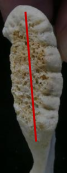
\includegraphics[scale = 0.75]{plataforma_dorsal_presente.png} & 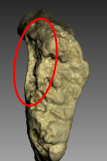
\includegraphics[scale = 0.75]{bisel_ventral_en_proceso_formacion.png} &   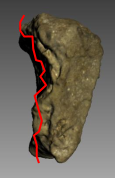
\includegraphics[scale = 0.75]{borde_ventral_muchas_excrecencias.png} \\ \hline
	\end{tabular}%
}
	\caption{Algunos ejemplos de las características consideradas por Todd.}\label{table:caracteristicas_todd}
\end{table}

Observando estas características Todd proponía una clasificación en diez fases:

\begin{itemize}
	\item Fase 1: 19 años.
	\item Fase 2: De 20 a 21 años.
	\item Fase 3: De 22 a 24 años.
	\item Fase 4: De 25 a 26 años.
	\item Fase 5: De 27 a 30 años.
	\item Fase 6: De 31 a 34 años.
	\item Fase 7: De 35 a 39 años.
	\item Fase 8: De 40 a 44 años.
	\item Fase 9: De 45 a 49 años.
	\item Fase 10: Más de 50 años.
\end{itemize}

Como era de esperar, podemos ver que las fases de edad más tempranas son más fáciles de asignar y los rangos de edad son más pequeños, mientras que en las fases más avanzadas los rangos de edad son mucho mayores, llegando a la última fase de más de 50 años, que aunque hoy en día nos parezca que gran parte de la población se asignaría a esa fase, en la época que Todd propuso esta clasificación la esperanza de vida era mucho menor.

En este trabajo propondremos una forma de automatizar este proceso de forma que sirva de ayuda al forense de cara a realizar su trabajo utilizando técnicas de inteligencia artificial y aprendizaje automático.

\subsubsection{Conjunto de datos}

Uno de los principales inconvenientes de este problema es que, como podemos ver, tenemos un gran número de características, de posibles valores para dichas características y de clases que asignar a cada dato, por lo que tendremos que buscar formas de reducir la dimensionalidad del problema.

Por otro lado, es muy dificil obtener un buen conjunto de datos para este problema. En nuestro caso utilizaremos un conjunto de datos clasificado manualmente por el Laboratorio de Antropología Física de la Universidad de Granada\cite{laboratorioForenseUGR}.

Este conjunto está formado por datos tomados de ambas lateralidades de la sínfisis púbica, siendo en total 892 datos distribuidos en los diez rangos de edades propuestos por Todd.

\begin{figure}[H]
	\centering
	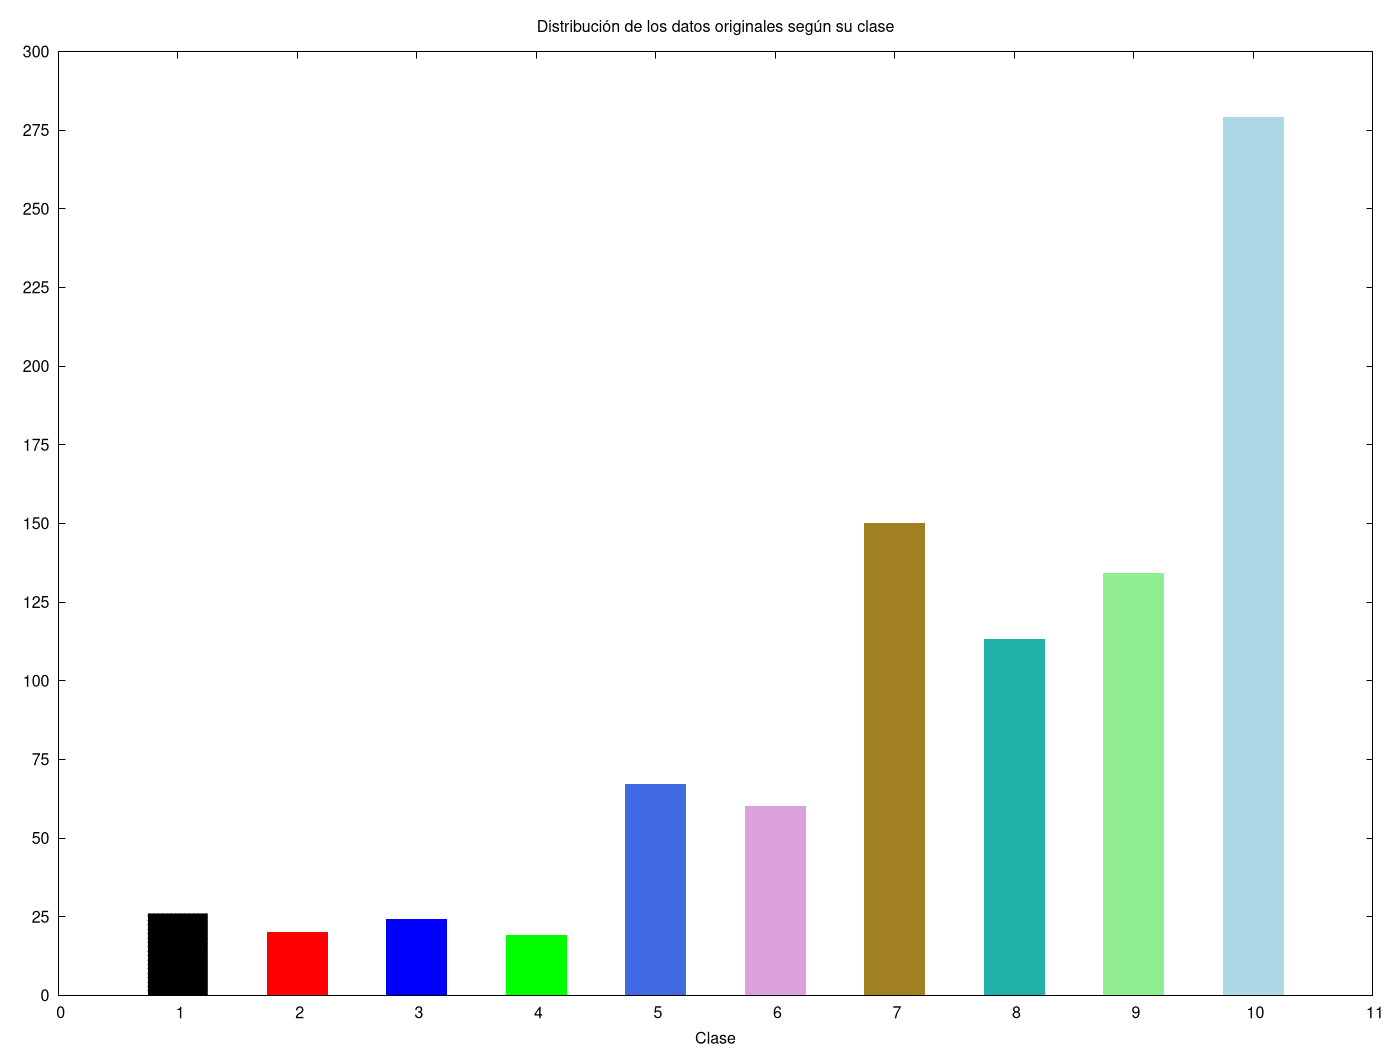
\includegraphics[scale = 0.30]{num_elementos_fase_original.png}
	\caption{Número de datos por cada clase con el conjunto de datos completo.}
	\label{fig:conteo_original}

\end{figure}

Como vemos, este conjunto de datos se encuentra claramente desbalanceado, hay muchas más muestras de las clases de edad más avanzada que de edades más bajas, además de contar con muy pocos en la mayoría de clases. Más adelante veremos como podemos solucionar estos problemas utilizando técnicas de sobremuestreo.

\subsection{Motivación}

Este trabajo está motivado ya que, aunque en los últimos años diversos modelos son capaces de obtener buenos resultados en esta clase de problemas, los modelos actuales apenas son interpretables por los expertos y esto no les permite utilizar estos modelos para avanzar en las técnicas de estimación de la edad a partir de restos óseos.

Por este motivo aparece la Inteligencia Artificial Explicable, y utilizando este tipo de técnicas intentaremos resolver el problema para que el experto sea capaz de entender y razonar como funciona el modelo.


\subsubsection{Inteligencia Artificial Explicable}

En la última década, gracias a los avances en la potencia computación, los distintos modelos de aprendizaje automático como las redes neuronales han revolucionado la inteligencia artificial. Estos nuevos modelos, a pesar de obtener resultados impensables con modelos clásicos, son demasiado complejos como para comprender la forma en la que funcionan internamente. Por este motivo ha aparecido el concepto de Inteligencia Artificial Explicable \cite{XAI} (XAI de sus siglas en inglés).

La inteligencia artificial explicable trata de expresar modelos de inteligencia artificial de una forma simple e interpretable. Con esto se busca que no solo los desarrolladores de dichos modelos sean capaces de comprobar y validar como funciona el modelo, sino que los usuarios sean capaces de entender a grandes rasgos como funciona, ya que en muchas ocasiones han de ser capaces de interpretar las decisiones del modelo para realizar su trabajo.

En este trabajo, debido a la complejidad del problema, así como que el experto que utilizará los resultados del modelo ha de ser capaz de interpretar, validar, y tomar decisiones con los resultados del modelo, se buscará obtener un modelo simple y fácilmente interpretable.


\subsection{Objetivos}

Tras introducir el problema, comentar los principales retos que nos podemos encontrar y orientar que tipo de solución buscamos, podemos distinguir estos claros objetivos:

\begin{enumerate}
	\item Reducir la dimensionalidad del problema.
	\item Equilibrar el número de datos de cada clase, así como obtener nuevos datos para las clases minoritarias.
	\item Estudiar, desarrollar y entrenar modelos que permitan una fácil interpretación.
\end{enumerate}


\newpage


\section{Estado del arte y antecedentes}

\subsection{Estado del arte del problema a tratar}

El problema de la estimación de la edad a partir de restos óseos es un problema que ya se ha tratado en distintas ocasiones, desde modificaciones a la propuesta de Todd, propuestas de como automatizar la estimación utilizando las características que proponía Todd, hasta estudios que utilizaban técnicas de visión por computador para recoger y procesar las características de los restos.

En 1990, J. M. Suchey y S. Brooks propusieron una modificación a la propuesta de Todd \cite{sucheyBrooks}, en la que evaluaban $1225$ restos óseos y llegaban a la conclusión de que era posible reducir las diez fases propuestas por Todd a seis fases, modificando el criterio de cada una de las fases y añadiendo cierto error marginal, aunque con un $95\%$ de confianza con los nuevos intervalos propuestos. Esta modificación es una de las más aceptadas por la comunidad científica, aunque la mayor parte de trabajos siguen utilizando las fases propuestas por Todd.

Uno de los más relevantes es un estudio publicado en el año 2015 en la revista \textit{Journal of forensic sciences} \cite{modelandoHuesos3D}, en el que se escaneaban los restos tomados como muestras para la variación de la sínfisis púbica y con esta variación realizar la estimación de la edad utilizando un modelo de regresión lineal y las seis fases propuestas por Suchey y Brooks. El conjunto de datos utilizado en este experimento se compone de $41$ esqueletos de personas estadounidenses y logran obtener una raíz del error cuadrático medio de unos $17.15$ años.

Ese mismo año, los mismos autores presentaron una mejora \cite{mejoraModelandoHuesos3D} en la que, en lugar de utilizar la variación total de la sínfisis púbica, utilizaban la flexión de un plano de forma que dicho plano coincida con la superficie del hueso. De esta forma, utilizando un conjunto de datos similar a su experimento anterior y la curvatura de la sínfisis púbica entrenaron un modelo de regresión lineal con el que obtuvieron una raíz del error cuadrático medio de unos $19$ años.

A finales de 2015, Beatrix Dudzik y Natalie R. Langley, de la Universidad de Tennessee y la Universidad Lincoln Memorial, propusieron \cite{componentBased} varios modelos basados en árboles de decisión y regresión logística multinomial. Para estos experimentos utilizaron 5 características de la sínfisis púbica de 47 individuos de entre 18 y 40 años. Obtuvieron muy buenos resultados, con una tasa de acierto del $94\%$ aunque solo utilizaban 3 de las 6 fases propuestas por Suchey y Brooks.


Más adelante, en 2018, varios investigadores de la República Checa publicaron un trabajo \cite{estimacionHuesosCadera} en el que, con un conjunto de $941$ restos óseos de personas de distinta raza entre 19 y 100 años, utilizando datos de los huesos de la cadera estudiaban las características comunes y las que diferenciaban las distintas edades, y consideraban 9 modelos distintos para realizar una estimación, desde un sistema de puntuación tradicional, utilizando la variación entre los huesos, distintos de regresión lineal, árboles de decisiones o redes neuronales artificiales. De estos modelos se llega a la conclusión que el mejor es un modelo de regresión multinomial, con el que obtienen una raíz del error cuadrático medio de unos $12.5$ años.

En 2017 investigadores de la Universidad de Granada publicaron un artículo preliminar de cara a obtener un modelo descriptivo basado en reglas con el que realizar la estimación de la edad a partir de la sínfisis púbica \cite{fuzzyAgeEstimation}. Utilizando $74$ muestras clasificadas manualmente consiguen entre 17 y 20 reglas utilizando árboles de decisión difusos que consiguen un error absoluto medio de $1.68$ años, aunque el resultado no es totalmente fiable debido a que no consiguen reglas para algunas fases propuestas por Todd.

Más adelante, en 2021, este mismo equipo con la ayuda de investigadores de la Universidad de Cordoba publicaron una continuación de su estudio \cite{NSLVOrdAge}. En este caso, utilizando el mismo conjunto de datos que utilizaremos nosotros, aplicando técnicas de balanceo y sobremuestreo de datos para resolver problemas relativos a dicho conjunto de datos, han enfocado el problema como un problema de clasificación ordinal. Utilizando el software NSLVOrd \cite{NSLVOrd}, un algoritmo de clasificación ordinal basado en el enfoque de aprendizaje de reglas de forma iterativa, publicando por investigadores de la Universidad de Granada en 2016, son capaces de obtener una raíz del error cuadrático medio de $12.34$ años utilizando 34 reglas para las distintas fases. Este es, hasta este momento, el mejor resultado del estado del arte de este problema, y además en este estudio se discute sobre la importancia de las características a observar en la sínfisis púbica propuestas por Todd, llegando a la conclusión de que ciertas características nunca se utilizan, y por lo tanto no entran en juego a la hora de realizar la estimación de la edad.

\subsection{Programación Genética y regresión simbólica}

La Programación Genética apareció como una adaptación de los algoritmos genéticos para representar programas de ordenador como cromosomas en una estructura de árbol. A pesar de que su aparición fue en 1985 no fue hasta principios de 1990 cuando este método comenzo a ser más utilizado gracias a John Koza \cite{kozaGP}.

La forma en la que la Programación Genética expresa los cromosomas permite resolver problemas de distintos tipos dando soluciones sencillas de interpretar, por este motivo este algoritmo y sus variaciones han sido bastante utilizadas.

Uno de los primeros trabajos fue de publicado por P. A. Whigham en 1995 \cite{PGgramaticas}, en el que se proponía utilizar una gramática inicial libre del contexto para generar expresiones a utilizar en el algoritmo de Programación Genética, y que el entrenamiento del algoritmo fuera capaz de completar la gramática y ampliándola con nuevas reglas, siendo un claro ejemplo de aprendizaje incremental.

Ese mismo año investigadores de la Universidad de Georgia publicaban un artículo \cite{primerGAP} en el que proponían utilizar Programación Genética para hacer regresión simbólica, es decir, aprender una fórmula matemática estructurada como un árbol, en este trabajo se mencionan los principales problemas de Programación Genética para ser aplicada a regresión simbólica y por eso se propone una modificación del algoritmo original, que será un híbrido entre Programación Genética y un Algoritmo Genético, de ahí el nombre GA-P (Genetic Algorithm-Programming).


Más adelante esta variación de Programación Genética se utilizará en diversos artículos, como el publicado por investigadores de la Universidad de Oviedo y la Universidad de Granada en 1999 \cite{GAPredElectrica}, donde utilizando este algoritmo consiguen unos resultados bastante buenos en dos problemas reales aplicando regresión simbólica.

Un año más tarde, en el año 2000, aunque ya se podían encontrar trabajos en los que se utilizaba Programación Genética y algunas variantes de cara a realizar regresión simbólica, dos investigadores del Laboratorio Nacional de Computación Científica de Brasil publican un artículo \cite{PGregresionSimbolica} donde explican como utilizar Programación Genética en regresión simbólica, explicando los distintos operadores necesarios.

En el año 2000, también investigadores de la Universidad de Granada, publicaron un trabajo donde utilizan GA-P para aprender consultas booleanas \cite{GAPFormulasBooleanas} en el que demuestran la versatilidad del algoritmo para distintos problemas, además de que las soluciones obtenidas son fácilmente interpretables.


%\subsection{Sistemas basados en reglas}


\section{Propuesta}


\subsection{Conjunto de datos a utilizar}

\subsection{Planificación temporal}


\section{Conclusiones}

En este trabajo hemos introducido un problema real y de gran interés que se lleva investigando durante un largo periodo de tiempo. Hemos revisado su estado del arte para entender el punto en el que se encuentra el problema, así como los distintos métodos y enfoques que se han propuesto para resolverlo. Tras esto, se ha propuesto utilizar un tipo de algoritmo evolutivo que nos permite obtener resultados fácilmente interpretables además de una introducción general a los distintos tipos de algoritmos evolutivos, explicado en profundidad la variante concreta que hemos utilizado así como distintas propuestas y mejoras sobre esta. Hemos explicado el funcionamiento de regresión simbólica aplicada al problema y realizado un estudio y aplicación de técnicas de sobremuestreo de datos para poder mejorar el conjunto de datos utilizado debido al gran desafío de obtener un conjunto de datos completo para este problema.

Más en detalle, se ha realizado un estudio del problema de la estimación de la edad a partir de los huesos del pubis, revisando la propuesta original de Thomas Wingate Todd, así como distintos enfoques que surgieron a partir de esta propuesta, como los de Gilbert y McKern, llegando a la conclusión de que se utilizará la propuesta de Gilbert y McKern de cara a enfocar el problema como un problema de regresión pero utilizando las características propuestas por Todd de cara a no eliminar grados de libertad en las características. Tras discutir la importancia de resolver este problema en el ámbito forense, se ha realizado una introducción a la inteligencia artificial explicable (XAI) y porqué en este problema en concreto el encontrar una solución interpretable es de gran interés, permitiendo a los forenses encontrar nuevas relaciones entre las características del pubis para poder mejorar su trabajo.

Tras esto, se ha discutido sobre la dificultad de encontrar un buen conjunto de datos que represente a todas las posibles edades de cara a poder obtener un modelo que sea capaz de generalizar los resultados sin importar la entrada y la necesidad de aplicarlo sobre nuestro conjunto de datos, llegando a analizar técnicas de sobremuestreo, centrándonos en SMOTE y sus variantes debido a sus buenos resultados en el estado del arte, así como sus adaptaciones a regresión debido al enfoque que se le ha dado al problema en este trabajo.

Por último se ha presentado una propuesta de algoritmo evolutivo cuyos resultados sean fácilmente interpretables y se pueda aplicar regresión simbólica con el fin de no solo aprender las constantes para ajustar la expresión, sino para aprender también la forma de la expresión, Programación Genética. Se ha realizado una introducción a algoritmos evolutivos, así como a las distintas variantes existentes, explicado en profundidad el funcionamiento de Programación Genética, la utilizada en este trabajo, sus ventajas y desventajas, además de una variante para mejorar su funcionamiento en regresión simbólica, GA-P, haciendo un híbrido entre Programación Genética y un Algoritmo Genético.

Tras realizar los distintos experimentos sobre estos dos algoritmos, tanto con el conjunto de datos original como el conjunto con datos generados de forma sintética, hemos concluido que, aunque ciertas características propuestas por Todd no influyen en la estimación de la edad y corroborando este hecho con el estado del arte, el enfoque tomado ha sido un acierto, llegando a mejorar los resultados del estado del arte tanto con el conjunto de datos original como con el conjunto con datos sintéticos, obteniendo fórmulas simples y fácilmente interpretables.


\addcontentsline{toc}{section}{Referencias}

\begin{thebibliography}{9}


	\bibitem{todd}

	\href{https://onlinelibrary.wiley.com/doi/abs/10.1002/ajpa.1330030301}{T. W. Todd, “Age changes in the pubic bone,” American Journal of Physical Anthropology, vol. 3, no. 3, pp. 285–328, 1920.}



	\bibitem{XAI}

	\href{https://www.sciencedirect.com/science/article/pii/S1566253519308103?via%3Dihub}{Arrieta, A. B., Díaz-Rodríguez, N., Del Ser, J., Bennetot, A., Tabik, S., Barbado, A., ... \& Herrera, F. (2020). Explainable Artificial Intelligence (XAI): Concepts, taxonomies, opportunities and challenges toward responsible AI. Information Fusion, 58, 82-115.}


	\bibitem{laboratorioForenseUGR}

	Antropología Forense – LiveMetrics UGR. \url{https://livemetrics.ugr.es/laboratorio-singular/antropologia-forense/}

	\bibitem{sucheyBrooks}

	\href{https://link.springer.com/article/10.1007/BF02437238}{Brooks, S., \& Suchey, J. M. (1990). Skeletal age determination based on the os pubis: a comparison of the Acsádi-Nemeskéri and Suchey-Brooks methods. Human evolution, 5(3), 227-238.}

	\bibitem{modelandoHuesos3D}

	\href{https://onlinelibrary.wiley.com/doi/full/10.1111/1556-4029.12778}{Slice, D. E., \& Algee‐Hewitt, B. F. (2015). Modeling bone surface morphology: a fully quantitative method for age‐at‐death estimation using the pubic symphysis. Journal of forensic sciences, 60(4), 835-843.}

	\bibitem{mejoraModelandoHuesos3D}

	\href{https://onlinelibrary.wiley.com/doi/full/10.1002/ajpa.22797}{Stoyanova, D., Algee‐Hewitt, B. F., \& Slice, D. E. (2015). An enhanced computational method for age‐at‐death estimation based on the pubic symphysis using 3 D laser scans and thin plate splines. American journal of physical anthropology, 158(3), 431-440.}


	\bibitem{componentBased}

	\href{https://www.sciencedirect.com/science/article/pii/S0379073815003254}{Dudzik, B., \& Langley, N. R. (2015). Estimating age from the pubic symphysis: A new component-based system. Forensic science international, 257, 98-105.}

	\bibitem{estimacionHuesosCadera}

	\href{https://www.sciencedirect.com/science/article/pii/S0379073818301440}{Kotěrová, A., Navega, D., Štepanovský, M., Buk, Z., Brůžek, J., \& Cunha, E. (2018). Age estimation of adult human remains from hip bones using advanced methods. Forensic science international, 287, 163-175.}


	\bibitem{fuzzyAgeEstimation}

	\href{https://ieeexplore.ieee.org/abstract/document/8015760}{Villar, P., Alemán, I., Castillo, L., Damas, S., \& Cordón, O. (2017, July). A first approach to a fuzzy classification system for age estimation based on the pubic bone. In 2017 IEEE International Conference on Fuzzy Systems (FUZZ-IEEE) (pp. 1-6). IEEE.}

	\bibitem{NSLVOrdAge}

	Gámez-Granados, J. C., Irurita, J., Pérez, R., González, A., Damas, S., Alemán, I. \& Cordón, O. Automating Todd’s Age Estimation Method from the Pubic Bone with Explainable Machine Learning

	\bibitem{NSLVOrd}

	\href{https://www.sciencedirect.com/science/article/pii/S0888613X16300706}{Gámez, J. C., García, D., González, A., \& Pérez, R. (2016). Ordinal classification based on the sequential covering strategy. International Journal of Approximate Reasoning, 76, 96-110.}

	\bibitem{kozaGP}

	\href{https://mitpress.mit.edu/books/genetic-programming}{Koza, J. R., \& Koza, J. R. (1992). Genetic programming: on the programming of computers by means of natural selection (Vol. 1). MIT press.}

	\bibitem{PGgramaticas}

	\href{https://www.researchgate.net/profile/Pa-Whigham/publication/2450222_Grammatically-based_Genetic_Programming/links/55c3c89908aebc967df1b765/Grammatically-based-Genetic-Programming.pdf}{Whigham, P. A. (1995, July). Grammatically-based genetic programming. In Proceedings of the workshop on genetic programming: from theory to real-world applications (Vol. 16, No. 3, pp. 33-41).}

	\bibitem{primerGAP}

	\href{https://ieeexplore.ieee.org/stamp/stamp.jsp?tp=&arnumber=393137}{Howard, L. M., \& D'Angelo, D. J. (1995). The GA-P: A genetic algorithm and genetic programming hybrid. IEEE expert, 10(3), 11-15.}

	\bibitem{GAPredElectrica}

	\href{https://link.springer.com/article/10.1023/A:1008384630089}{Cordón, O., Herrera, F., \& Sánchez, L. (1999). Solving electrical distribution problems using hybrid evolutionary data analysis techniques. Applied Intelligence, 10(1), 5-24.}


	\bibitem{PGregresionSimbolica}

	\href{https://ieeexplore.ieee.org/document/889734}{Augusto, D. A., \& Barbosa, H. J. (2000, November). Symbolic regression via genetic programming. In Proceedings. Vol. 1. Sixth Brazilian Symposium on Neural Networks (pp. 173-178). IEEE.}

	\bibitem{GAPFormulasBooleanas}

	\href{https://upcommons.upc.edu/handle/2099/3586}{Cordón García, O., Moya Anegón, F. D., \& Zarco Fernández, C. (2000). A GA-P algorithm to automatically formulate extended Boolean queries for a fuzzy information retrieval system. Mathware \& soft computing. 2000 Vol. 7 Núm. 2 [-3].}

	\bibitem{revisionSMOTE}

	\href{https://www.jair.org/index.php/jair/article/view/11192}{Fernández, A., Garcia, S., Herrera, F., \& Chawla, N. V. (2018). SMOTE for learning from imbalanced data: progress and challenges, marking the 15-year anniversary. Journal of artificial intelligence research, 61, 863-905.}

	\bibitem{propuestaADASYN}

	\href{https://ieeexplore.ieee.org/abstract/document/4633969}{He, H., Bai, Y., Garcia, E. A., \& Li, S. (2008, June). ADASYN: Adaptive synthetic sampling approach for imbalanced learning. In 2008 IEEE international joint conference on neural networks (IEEE world congress on computational intelligence) (pp. 1322-1328). IEEE.}

	\bibitem{propuestaGilbert}

	\href{https://onlinelibrary.wiley.com/doi/abs/10.1002/ajpa.1330380109}{Gilbert, B. M., \& McKern, T. W. (1973). A method for aging the female os pubis. American Journal of Physical Anthropology, 38(1), 31-38.}


	\bibitem{OpenMP}

	OpenMP ARB. «Home». OpenMP, \url{https://www.openmp.org}.

	\bibitem{gdb}

	GDB: The GNU Project Debugger. \url{https://www.gnu.org/software/gdb/}.

	\bibitem{valgrind}

	Valgrind Home. \url{https://valgrind.org/}.

	\bibitem{gtest}

	google/googletest. 2015. Google, 2021. GitHub, \url{https://github.com/google/googletest}.

	\bibitem{git}

	Git. \url{https://git-scm.com/}.

	\bibitem{BL-SMOTE}

	\href{https://link.springer.com/chapter/10.1007/11538059_91}{Han, H., Wang, W. Y., \& Mao, B. H. (2005, August). Borderline-SMOTE: a new over-sampling method in imbalanced data sets learning. In International conference on intelligent computing (pp. 878-887). Springer, Berlin, Heidelberg.}

	\bibitem{SMOTE}

	\href{https://www.jair.org/index.php/jair/article/view/10302}{Chawla, N. V., Bowyer, K. W., Hall, L. O., \& Kegelmeyer, W. P. (2002). SMOTE: synthetic minority over-sampling technique. Journal of artificial intelligence research, 16, 321-357.}

	\bibitem{imblearnBLSMOTE}

	BorderlineSMOTE — Imbalanced Learn Version 0.8.0. \url{https://imbalanced-learn.org/stable/references/generated/imblearn.over_sampling.BorderlineSMOTE.html}.


\end{thebibliography}


\end{document}
